\documentclass{article}[12pt]
\usepackage{color}
\usepackage[normalem]{ulem}
\usepackage{times}
\usepackage{fullpage}
\usepackage{amsmath}
\usepackage{amssymb}
\usepackage{listings}
\usepackage{tikz}
\def \R {\mathbb R}
\def \imp {\Longrightarrow}
\def \eps {\varepsilon}
\def \Inf {{\sf Inf}}
\newenvironment{proof}{{\bf Proof.  }}{\hfill$\Box$}
\newtheorem{theorem}{Theorem}[section]
\newtheorem{definition}{Definition}[section]
\newtheorem{corollary}{Corollary}[section]
\newtheorem{lemma}{Lemma}[section]
\newtheorem{claim}{Claim}[section]
\setlength {\parskip}{2pt}
\setlength{\parindent}{0pt}

\newcommand{\headings}[4]{\noindent {\bf Assignment 13 CME241} \hfill {{\bf Author:} Nicolas Sanchez} \\
{} \hfill {{\bf Due Date:} #2} \\

\rule[0.1in]{\textwidth}{0.025in}
}

\newcommand{\klnote}[1]{{\color{red} #1}}
\newcommand{\klsout}[1]{{\color{red} \sout{#1}}}

\begin{document}

\headings{\#1}{Tuesday, October 8, 10:30am}\section{} 

\section{RL Control}
We implement the three types of RL Control with the code included below:
\begin{lstlisting}
def mc_control(
        mdp: MarkovDecisionProcess[S, A],
        states: Distribution[S],
        approx_0: FunctionApprox[Tuple[S, A]],
        gamma: float,
        eps: Callable[[int], float],
        tolerance: float = 1e-6
) -> Iterator[FunctionApprox[Tuple[S, A]]]:

    q = approx_0
    p = markov_decision_process.policy_from_q(q, mdp)
    trace_count = 1
    while True:
        trace: Iterable[markov_decision_process.TransitionStep[S, A]] =\
            mdp.simulate_actions(states, p)


        q = q.update(
            ((step.state, step.action), step.return_)
            for step in returns(trace, gamma, tolerance)
        )

        p = markov_decision_process.policy_from_q(q, mdp, eps(trace_count))
        trace_count += 1
        yield q


def td_sarsa(
        mdp: MarkovDecisionProcess[S, A],
        states: Distribution[S],
        approx_0: FunctionApprox[Tuple[S, A]],
        gamma: float,
        episodes:int  = 1000,
        max_iter:int = 100000
) -> FunctionApprox[Tuple[S, A]]:
    q = approx_0
    iter_count = 0
    for episode_num in range(episodes):
        epsilon: float = 1.0 / (episode_num + 1)
        state: Cell = states.sample()
        
        # go through a full episode

        while(True):
            p = markov_decision_process.policy_from_q(q, mdp, epsilon)
            action = p.act(state).sample()
            next_state, reward = mdp.step(state,action).sample()            
            # end while loop if end of road
            if mdp.is_terminal(next_state):
                q = q.update([((state, action),reward)])
                break

            next_action = p.act(next_state).sample()
            q = q.update([( (state, action),reward+gamma*q((next_state,next_action)))])
            state = next_state
            iter_count += 1
            if iter_count > max_iter: break
        if iter_count > max_iter: break
    return q


def q_learning(
        mdp: MarkovDecisionProcess[S, A],
        states: Distribution[S],
        approx_0: FunctionApprox[Tuple[S, A]],
        gamma: float,
        episodes:int  = 1000,
        max_iter:int = 100000
) -> Iterator[FunctionApprox[Tuple[S, A]]]:
    q = approx_0
    iter_count = 0
    for episode_num in range(episodes):
        epsilon: float = 1.0 / (episode_num + 1)
        state: Cell = states.sample()
        # go through a full episode
        while(True):
            p = markov_decision_process.policy_from_q(q, mdp, epsilon)
            action = p.act(state).sample()
            next_state, reward = mdp.step(state,action).sample()
            
            # end while loop if end of road
            if mdp.is_terminal(next_state):
                q = q.update([((state, action),reward)])
                break

            next_reward = max(q((next_state, a)) for a in mdp.actions(next_state))
            q = q.update([( (state, action),reward+gamma*next_reward)])
            state = next_state
            iter_count += 1
            if iter_count > max_iter: break
        if iter_count > max_iter: break
    return q
\end{lstlisting}

We test out our implementation on the simple inventory problem and obtain almost the same policy for the three control statements:
\begin{figure}
  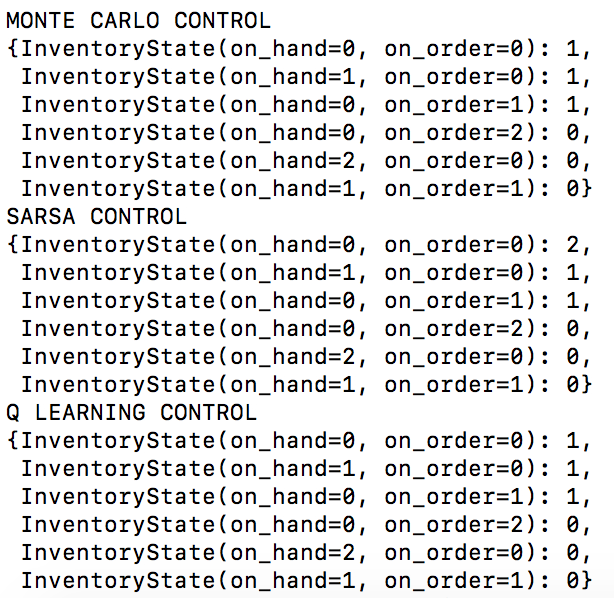
\includegraphics[width=0.5\linewidth]{Result_SIMDP.png}
  \caption{Convergence of three control methods}
  \label{fig:optPol1}
\end{figure}
\end{document}
